\documentclass[11pt]{article}
\usepackage[utf8]{inputenc}
\usepackage[dvips]{graphicx}
\usepackage{fancybox}
\usepackage{verbatim}
\usepackage{multirow,array}
\usepackage{latexsym}
\usepackage{alltt}
\usepackage{hyperref}
\usepackage{textcomp}
\usepackage{color}
\usepackage{amsmath}
\usepackage{amsfonts}
\usepackage{tikz}
\usepackage{float}
\usepackage[hmargin=3cm,vmargin=5.0cm]{geometry}
%\topmargin=0cm
\topmargin=-2cm
\addtolength{\textheight}{6.5cm}
\addtolength{\textwidth}{2.0cm}
%\setlength{\leftmargin}{-5cm}
\setlength{\oddsidemargin}{0.0cm}
\setlength{\evensidemargin}{0.0cm}


\begin{document}

\section*{Student Information } 
%Write your full name and id number between the colon and newline
%Put one empty space character after colon and before newline
Full Name :  Ozan Akın \\
Id Number :  2309599 \\

% Write your answers below the section tags

\section*{Answer 1}
\subsection*{a)}

\begin{figure}[H]
	\centering
	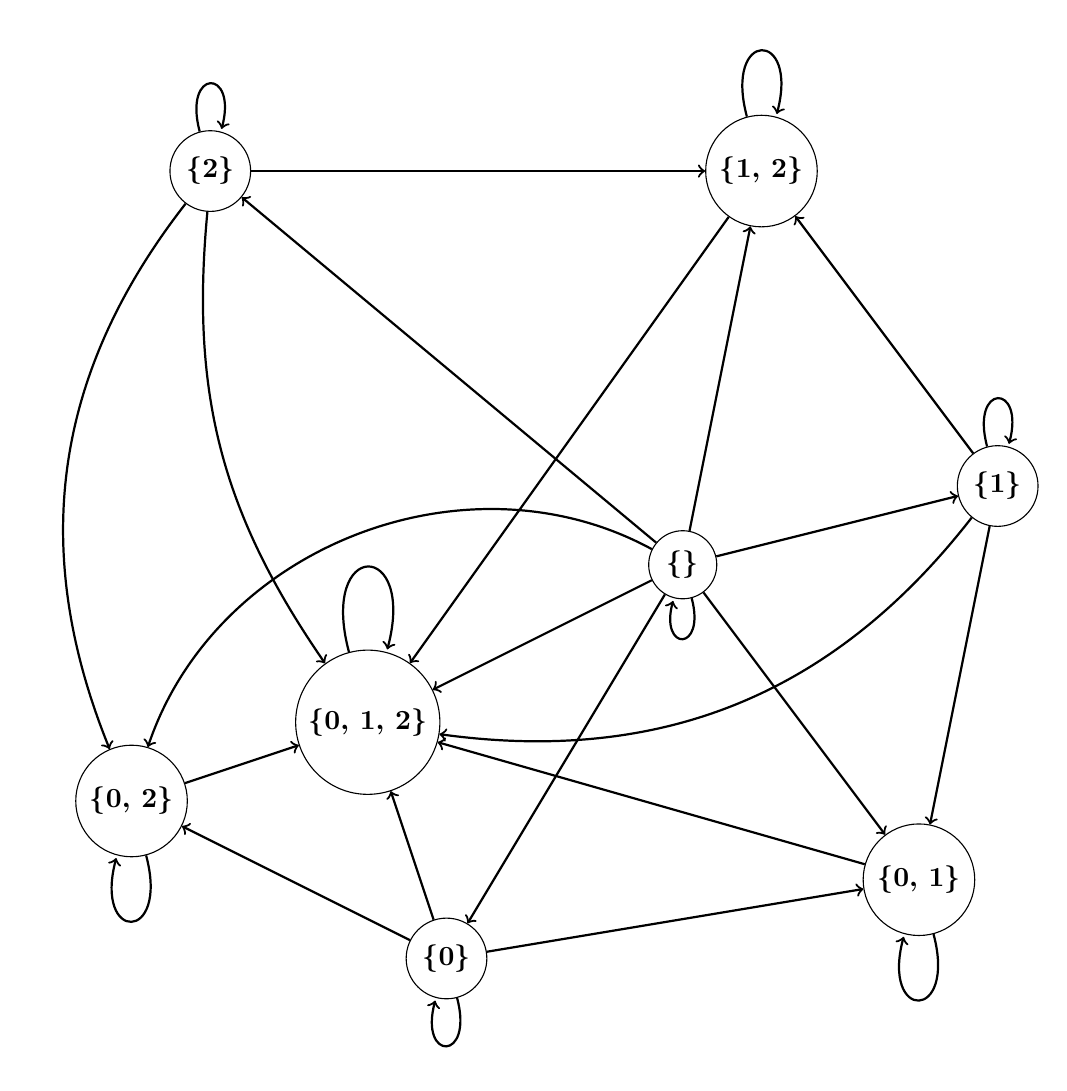
\begin{tikzpicture}
	
	\node[shape=circle,draw=black] (a) at (7, 5)    {\textbf{\{\}}};
	
	\node[shape=circle,draw=black] (b) at (4, 0)    {\textbf{\{0\}}};
	\node[shape=circle,draw=black] (c) at (11, 6)   {\textbf{\{1\}}};
	\node[shape=circle,draw=black] (d) at (1, 10)   {\textbf{\{2\}}};
	
	\node[shape=circle,draw=black] (e) at (10, 1)   {\textbf{\{0, 1\}}};
	\node[shape=circle,draw=black] (f) at (0, 2)    {\textbf{\{0, 2\}}};
	\node[shape=circle,draw=black] (g) at (8, 10)   {\textbf{\{1, 2\}}};
	
	\node[shape=circle,draw=black] (h) at (3, 3)    {\textbf{\{0, 1, 2\}}};
	
    \path[->, thick] (a) edge [loop below] (a);
    \path[->, thick] (b) edge [loop below] (b);
    \path[->, thick] (c) edge [loop above] (c);
    \path[->, thick] (d) edge [loop above] (d);
    \path[->, thick] (e) edge [loop below] (e);
    \path[->, thick] (f) edge [loop below] (f);
    \path[->, thick] (g) edge [loop above] (g);
    \path[->, thick] (h) edge [loop above] (h);
    
    \path[->, thick] (a) edge (b);
    \path[->, thick] (a) edge (c);
    \path[->, thick] (a) edge (d);
    \path[->, thick] (a) edge (e);
    \path[->, thick] (a) edge [bend right=50] (f);
    \path[->, thick] (a) edge (g);
    \path[->, thick] (a) edge (h);
    
    \path[->, thick] (b) edge (e);
    \path[->, thick] (b) edge (f);
    \path[->, thick] (b) edge (h);
    
    \path[->, thick] (c) edge (e);
    \path[->, thick] (c) edge (g);
    \path[->, thick] (c) edge [bend left=30] (h);
    
    \path[->, thick] (d) edge [bend right=30] (f);
    \path[->, thick] (d) edge (g);
    \path[->, thick] (d) edge [bend right=20] (h);
    
    \path[->, thick] (e) edge (h);
    \path[->, thick] (f) edge (h);
    \path[->, thick] (g) edge (h);
    
	\end{tikzpicture}
\end{figure}

\subsection*{b)}
    \begin{itemize}
        \item Definition 1 from section 9.6 of the textbook says "A relation R on a set S is called a partial ordering or partial order if it is reflexive, antisymmetric, and transitive. A set S together with a partial ordering R is called a partially ordered set, or poset, and is denoted by $(S, R)$. Members of S are called elements of the poset."
        \item Hence, we need to prove that graph is reflexive, antisymmetric, and transitive.
        \item Reflexivity: Since each element has a loop to itself, the graph is reflexive. 
        \item Antisymmetry: Since there is no edge such that edge which is opposite direction of an edge of two vertices, the graph is antisymmetric.
        \item Transitivity: Since there are some vertices such that there is at least one edge from and to the graph, such as \texttt{\{1\}} and \texttt{\{2\}} the graph is transitive.
        \item Since the graph is reflexive, antisymmetric, and transitive, $(S, R)$ is a poset.
    \end{itemize}{}

\subsection*{c)}
    \begin{itemize}
        \item Definition 3 from section 9.6 of the textbook says "If $(S, R)$ is a poset and every two elements of $S$ are comparable, $S$ is called a totally ordered or linearly ordered set, and R is called a total order".
        \item Since $(S, R)$ is a poset and we can compare two sets, $(S, R)$ is a total order.
    \end{itemize}{}

\subsection*{d)}

\begin{figure}[H]
	\centering
	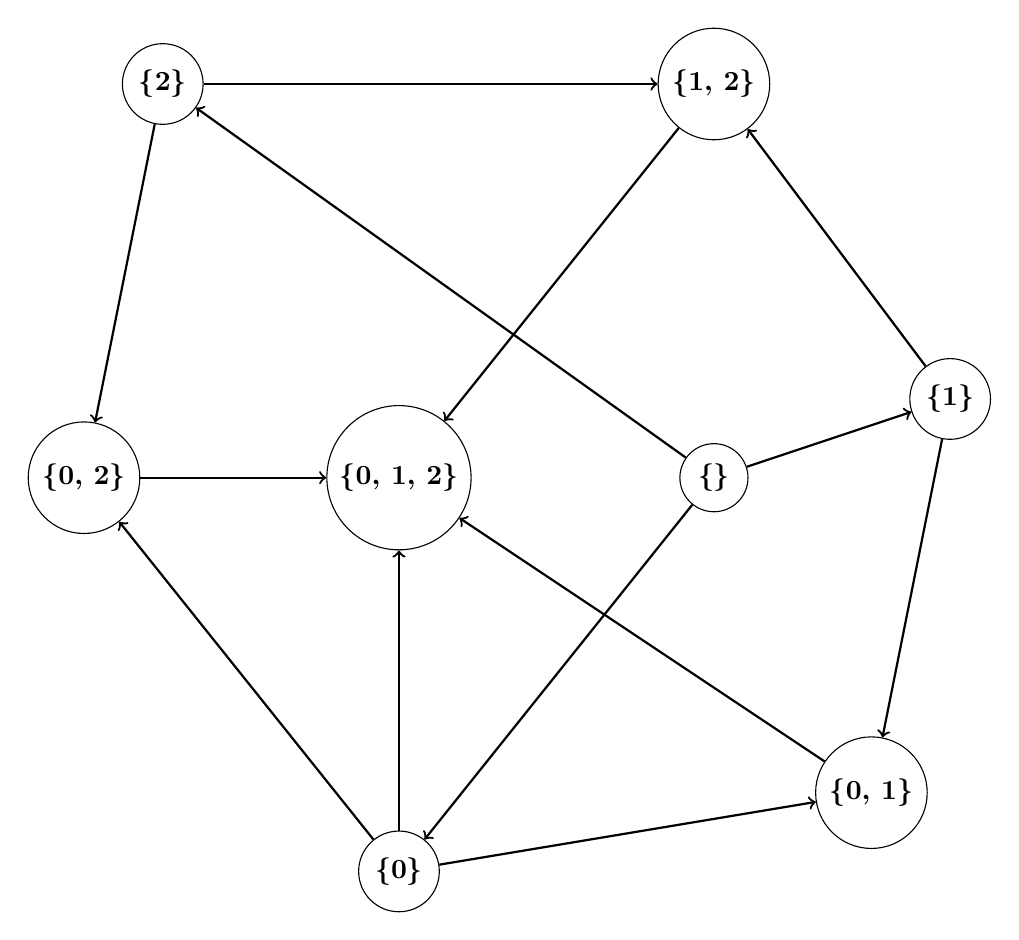
\begin{tikzpicture}
	
	\node[shape=circle,draw=black] (a) at (8, 5)    {\textbf{\{\}}};
	
	\node[shape=circle,draw=black] (b) at (4, 0)    {\textbf{\{0\}}};
	\node[shape=circle,draw=black] (c) at (11, 6)   {\textbf{\{1\}}};
	\node[shape=circle,draw=black] (d) at (1, 10)   {\textbf{\{2\}}};
	
	\node[shape=circle,draw=black] (e) at (10, 1)    {\textbf{\{0, 1\}}};
	\node[shape=circle,draw=black] (f) at (0, 5)    {\textbf{\{0, 2\}}};
	\node[shape=circle,draw=black] (g) at (8, 10)   {\textbf{\{1, 2\}}};
	
	\node[shape=circle,draw=black] (h) at (4, 5)   {\textbf{\{0, 1, 2\}}};
	
    \path[->, thick] (a) edge (b);
    \path[->, thick] (a) edge (c);
    \path[->, thick] (a) edge (d);
    
    \path[->, thick] (b) edge (e);
    \path[->, thick] (b) edge (f);
    \path[->, thick] (b) edge (h);
    
    \path[->, thick] (c) edge (e);
    \path[->, thick] (c) edge (g);
    
    \path[->, thick] (d) edge (f);
    \path[->, thick] (d) edge (g);
    
    \path[->, thick] (e) edge (h);
    \path[->, thick] (f) edge (h);
    \path[->, thick] (g) edge (h);
    
	\end{tikzpicture}
\end{figure}

\subsection*{e)}
    \begin{itemize}
        \item Lattice definition from section 9.6 of the textbook says "A partially ordered set in which every pair of elements has both a least upper bound and a greatest lower bound is called a lattice.
        \item Since the upper bound of the vertices \texttt{\{1\}} and \texttt{\{2\}} are not the same, $(S, R)$ is not a lattice.
    \end{itemize}{}
    
\pagebreak

\section*{Answer 2}
\subsection*{a)}
    \begin{table}[H]
        \centering
        \begin{tabular}{c|c}
             initial vertex & terminal vertices \\
             \hline
             a & \\
             b & a, c \\
             c & f \\
             d & c, d, e, g \\
             e & c, f, g \\
             f & b \\
             g & d
        \end{tabular}
    \end{table}{}

\subsection*{b)}
    \begin{figure}[H]
    $$  
        \begin{bmatrix}{}
            0 & 0 & 0 & 0 & 0 & 0 & 0 \\
            1 & 0 & 1 & 0 & 0 & 0 & 0 \\
            0 & 0 & 0 & 0 & 0 & 1 & 0 \\
            0 & 0 & 1 & 1 & 1 & 0 & 1 \\
            0 & 0 & 1 & 0 & 0 & 1 & 1 \\
            0 & 1 & 0 & 0 & 0 & 0 & 0 \\
            0 & 0 & 0 & 1 & 0 & 0 & 0
        \end{bmatrix}{} 
    $$
    \end{figure}{}

\subsection*{c)}
    \begin{table}[H]
        \centering
        \begin{tabular}{c|c|c}
             vertex & in-degrees count & out-degrees count \\
             \hline
             a & 2 & 0 \\
             b & 1 & 2 \\
             c & 3 & 1 \\
             d & 2 & 5 \\
             e & 1 & 3 \\
             f & 2 & 1 \\
             g & 2 & 1
        \end{tabular}
    \end{table}{}

\subsection*{d)}
    
    \begin{itemize}
        \item $b \rightarrow c \rightarrow f \rightarrow b \rightarrow a$
        \item $d \rightarrow g \rightarrow d \rightarrow e \rightarrow c$
        \item $d \rightarrow c \rightarrow f \rightarrow b \rightarrow a$
        \item $e \rightarrow f \rightarrow b \rightarrow c \rightarrow f$
        \item $d \rightarrow e \rightarrow c \rightarrow f \rightarrow b$
        \item $e \rightarrow g \rightarrow d \rightarrow c \rightarrow f$
    \end{itemize}{}

\pagebreak

\subsection*{e)}

    \begin{itemize}
        \item $b \rightarrow c \rightarrow f \rightarrow b$
        \item $c \rightarrow f \rightarrow b \rightarrow c$
        \item $d \rightarrow d \rightarrow g \rightarrow d$
        \item $d \rightarrow e \rightarrow g \rightarrow d$
        \item $d \rightarrow g \rightarrow d \rightarrow d$
        \item $e \rightarrow g \rightarrow d \rightarrow e$
        \item $f \rightarrow b \rightarrow c \rightarrow f$
        \item $g \rightarrow d \rightarrow d \rightarrow g$
        \item $g \rightarrow d \rightarrow e \rightarrow g$
    \end{itemize}{}

\subsection*{f)}
    
    \begin{itemize}
        \item Since there is no path from \textit{a to b}, we can say that the graph is \textit{not strongly connected}.
        \item By using Definition 5 from the textbook Section 10.4, we can say that if there is a path between every two vertices in underlying undirected graph, the directed graph is \textit{weakly connected}.
        
            \begin{figure}[H]
            	\centering
            	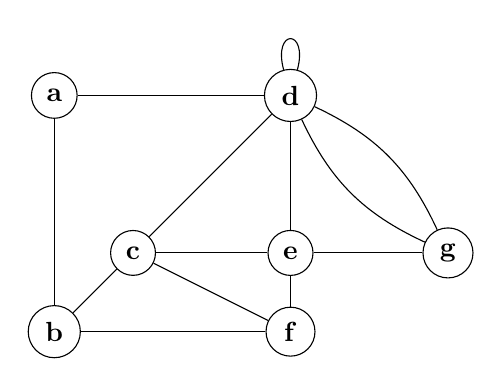
\begin{tikzpicture}[every loop/.style={}]
            	
            	\node[shape=circle,draw=black] (a) at (0, 3)     {\textbf{a}};
            	\node[shape=circle,draw=black] (b) at (0, 0)     {\textbf{b}};
            	\node[shape=circle,draw=black] (c) at (1, 1)     {\textbf{c}};
            	\node[shape=circle,draw=black] (d) at (3, 3)     {\textbf{d}};
            	\node[shape=circle,draw=black] (e) at (3, 1)     {\textbf{e}};
            	\node[shape=circle,draw=black] (f) at (3, 0)     {\textbf{f}};
            	\node[shape=circle,draw=black] (g) at (5, 1)     {\textbf{g}};
            
            	\path[-] (b) edge (a);
            	\path[-] (b) edge (c);
            	\path[-] (c) edge (f);
            	\path[-] (d) edge [loop above] (d);
            	\path[-] (d) edge (c);
            	\path[-] (d) edge (e);
            	\path[-] (d) edge (a);
            	\path[-] (d) edge [bend right=20] (g);
            	\path[-] (e) edge (c);
            	\path[-] (e) edge (f);
            	\path[-] (e) edge (g);
            	\path[-] (f) edge (b);
            	\path[-] (g) edge [bend right=20] (d);
            	\end{tikzpicture} 
            	
            	\caption{underlying undirected graph}
            	\label{g2}
            \end{figure}
        
        \item Since all vertices are connected a vertex except themselves, we can create a path between every two vertices.
        \item Hence, the direct graph is weakly connected.
    \end{itemize}{}

\subsection*{g)}
    \begin{itemize}
        \item the vertex a
        \item the subgraph containing vertices b, c, f, and edges $(b \rightarrow c)$, $(c \rightarrow f)$, $(f \rightarrow b)$
        \item the subgraph containing vertices d, e, g, and edges $(d \rightarrow e)$, $(e \rightarrow g)$, $(g \rightarrow d)$, $(d \rightarrow g)$
    \end{itemize}{}
    
\subsection*{h)}

    \begin{itemize}
        \item By using matrix from part b, we can generate adjacency matrix for subgraph H, the matrix $A$.
            \begin{figure}[H]
            $$  
                \begin{bmatrix}{}
                    1 & 1 & 0 & 1 \\
                    0 & 0 & 1 & 1 \\
                    0 & 0 & 0 & 0 \\
                    1 & 0 & 0 & 0
                \end{bmatrix}{} 
            $$
            \end{figure}{}
        \item Since we want to find different paths from d to g with length 3, by using Theorem 2 from the section 10.4 of the textbook, we need $A^3$.
            \begin{figure}[H]
            $$  
                \begin{bmatrix}{}
                    4 & 2 & 1 & 3 \\
                    1 & 1 & 0 & 1 \\
                    0 & 0 & 0 & 0 \\
                    2 & 1 & 1 & 2
                \end{bmatrix}{} 
            $$
            \end{figure}{}
        \item Hence, there are 3 different paths from d to g.
    \end{itemize}{}

\section*{Answer 3}
    First, let's find degrees of vertices for the graph $G$.
    \begin{table}[H]
        \centering
        \begin{tabular}{c|c|c|c|c|c|c|c}
             a & b & c & d & e & f & g & h \\
             \hline
             2 & 3 & 2 & 5 & 4 & 2 & 2 & 2 
        \end{tabular}
    \end{table}{}
    
\subsection*{a)}
    \begin{itemize}
        \item Theorem 2 from the section 10.5 of the textbook says "A connected multigraph has an Euler path but not an Euler circuit if and only if it has exactly
two vertices of odd degree."
        \item Since, only the vertices \texttt{b and d} have odd degree, others have even degree, the graph G has an Euler path.
    \end{itemize}{}
    
\subsection*{b)}
    \begin{itemize}
        \item Theorem 1 from the section 10.5 of the textbook says "A connected multigraph with at least two vertices has an Euler circuit if and only if each of its vertices has even degree."
        \item From the both part a and theorem 1, we can conclude that the graph G has not an Euler circuit since there are vertices with odd degree such as \texttt{b and d}.
        \item Hence, the graph G has not a Euler circuit.
    \end{itemize}{}
    
\subsection*{c)}
    \begin{itemize}
        \item Definition 2 from the section 10.5 of the textbook says "A simple path in a Graph G that passes through every vertex exactly once is called a Hamilton Path."
        \item Since we cannot create a path that passes through every vertex without passing the vertices \texttt{d and e} twice, we cannot create a path passes through every vertex only once.
        \item Hence, the graph G has not a Hamilton path.
    \end{itemize}{}
    
\subsection*{d)}
    \begin{itemize}
        \item Theorem 2 from the section 10.5 of the textbook (Dirac’s Theorem) says "If G is a simple graph with n vertices with $n \ge 3$ such that the degree of every vertex in G is at least $n/2$, then G has a Hamilton circuit."
        \item Since the number vertices is $\mathbf{8}$, the degree of every vertex in G must be $d \ge 4$.
        \item But the vertices \texttt{a, c, f, g and h} have degree of 2. Hence, the graph G has not a Hamilton circuit.
    \end{itemize}{}
    
\section*{Answer 4}
    \begin{itemize}
        \item To find whether these graphs are isomorphic, we can use adjacency matrices. If these matrices are identical, then the graphs are isomorphic.
        \item Adjacency matrix for graph $G$.
            \begin{figure}[H]
            $$  
                \begin{bmatrix}{}
                    0 & 1 & 0 & 0 & 1 \\
                    1 & 0 & 1 & 0 & 0 \\
                    0 & 1 & 0 & 1 & 0 \\
                    0 & 0 & 1 & 0 & 1 \\
                    1 & 0 & 0 & 1 & 0
                \end{bmatrix}{} 
            $$
            \end{figure}{}
        \item Adjacency matrix for graph $G^{'}$.
            \begin{figure}[H]
            $$  
                \begin{bmatrix}{}
                    0 & 1 & 0 & 0 & 1 \\
                    1 & 0 & 1 & 0 & 0 \\
                    0 & 1 & 0 & 1 & 0 \\
                    0 & 0 & 1 & 0 & 1 \\
                    1 & 0 & 0 & 1 & 0
                \end{bmatrix}{} 
            $$
            \end{figure}{}
        \item Since these matrices are identical, these two graphs are isomorphic.
    \end{itemize}{}

\section*{Answer 5}
\subsection*{a)}
    \begin{itemize}
    
\item \textbf{Step 0}
\begin{figure}[H]
	\centering
	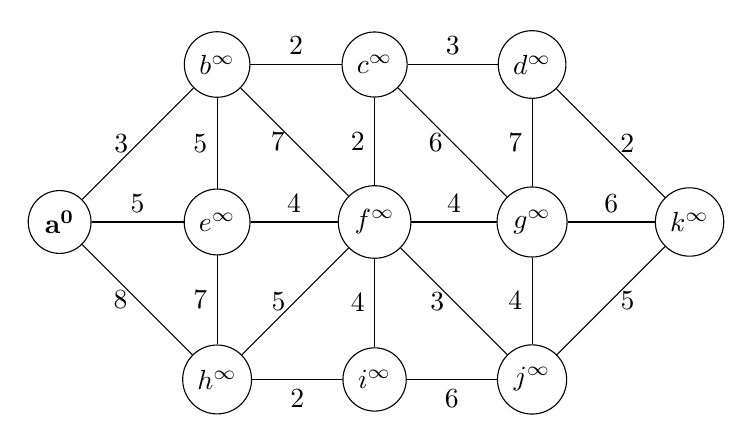
\begin{tikzpicture}
	\node[shape=circle,draw=black] (a) at (0, 2)     {\textbf{$\mathbf{a^0}$}};
	\node[shape=circle,draw=black] (b) at (2, 4)     {\textbf{$b^{\infty}$}};
	\node[shape=circle,draw=black] (c) at (4, 4)     {\textbf{$c^{\infty}$}};
	\node[shape=circle,draw=black] (d) at (6, 4)     {\textbf{$d^{\infty}$}};
	\node[shape=circle,draw=black] (e) at (2, 2)     {\textbf{$e^{\infty}$}};
	\node[shape=circle,draw=black] (f) at (4, 2)     {\textbf{$f^{\infty}$}};
	\node[shape=circle,draw=black] (g) at (6, 2)     {\textbf{$g^{\infty}$}};
	\node[shape=circle,draw=black] (h) at (2, 0)     {\textbf{$h^{\infty}$}};
	\node[shape=circle,draw=black] (i) at (4, 0)     {\textbf{$i^{\infty}$}};
	\node[shape=circle,draw=black] (j) at (6, 0)     {\textbf{$j^{\infty}$}};
	\node[shape=circle,draw=black] (k) at (8, 2)     {\textbf{$k^{\infty}$}};

	\path[-] (a) edge node[left]{3} (b);
	\path[-] (a) edge node[above]{5} (e);
	\path[-] (a) edge node[left]{8} (h);
	\path[-] (b) edge node[left]{5} (e);
	\path[-] (b) edge node[left]{7} (f);
	\path[-] (b) edge node[above]{2} (c);
	\path[-] (e) edge node[above]{4} (f);
	\path[-] (e) edge node[left]{7} (h);
	\path[-] (h) edge node[left]{5} (f);	
	\path[-] (h) edge node[below]{2} (i);	
	\path[-] (c) edge node[above]{3} (d);
	\path[-] (c) edge node[left]{6} (g);
	\path[-] (c) edge node[left]{2} (f);
	\path[-] (f) edge node[above]{4} (g);
	\path[-] (f) edge node[left]{3} (j);
	\path[-] (f) edge node[left]{4} (i);
	\path[-] (i) edge node[below]{6} (j);	
	\path[-] (d) edge node[right]{2} (k);
	\path[-] (d) edge node[left]{7} (g);
	\path[-] (g) edge node[above]{6} (k);
	\path[-] (g) edge node[left]{4} (j);
	\path[-] (j) edge node[right]{5} (k);
	\end{tikzpicture}
\end{figure}

\pagebreak

\item \textbf{Step 1}

Visiting node $a$.

\begin{figure}[H]
	\centering
	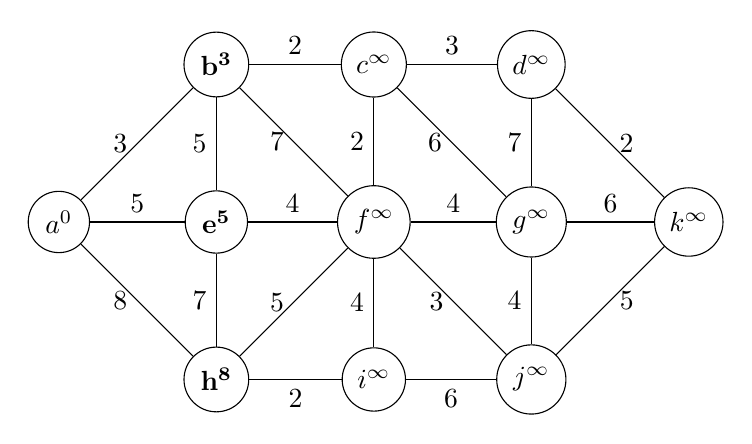
\begin{tikzpicture}
	\node[shape=circle,draw=black] (a) at (0, 2)     {\textbf{$a^0$}};
	\node[shape=circle,draw=black] (b) at (2, 4)     {\textbf{$\mathbf{b^3}$}};
	\node[shape=circle,draw=black] (c) at (4, 4)     {\textbf{$c^{\infty}$}};
	\node[shape=circle,draw=black] (d) at (6, 4)     {\textbf{$d^{\infty}$}};
	\node[shape=circle,draw=black] (e) at (2, 2)     {\textbf{$\mathbf{e^5}$}};
	\node[shape=circle,draw=black] (f) at (4, 2)     {\textbf{$f^{\infty}$}};
	\node[shape=circle,draw=black] (g) at (6, 2)     {\textbf{$g^{\infty}$}};
	\node[shape=circle,draw=black] (h) at (2, 0)     {\textbf{$\mathbf{h^8}$}};
	\node[shape=circle,draw=black] (i) at (4, 0)     {\textbf{$i^{\infty}$}};
	\node[shape=circle,draw=black] (j) at (6, 0)     {\textbf{$j^{\infty}$}};
	\node[shape=circle,draw=black] (k) at (8, 2)     {\textbf{$k^{\infty}$}};

	\path[-] (a) edge node[left]{3} (b);
	\path[-] (a) edge node[above]{5} (e);
	\path[-] (a) edge node[left]{8} (h);
	\path[-] (b) edge node[left]{5} (e);
	\path[-] (b) edge node[left]{7} (f);
	\path[-] (b) edge node[above]{2} (c);
	\path[-] (e) edge node[above]{4} (f);
	\path[-] (e) edge node[left]{7} (h);
	\path[-] (h) edge node[left]{5} (f);	
	\path[-] (h) edge node[below]{2} (i);	
	\path[-] (c) edge node[above]{3} (d);
	\path[-] (c) edge node[left]{6} (g);
	\path[-] (c) edge node[left]{2} (f);
	\path[-] (f) edge node[above]{4} (g);
	\path[-] (f) edge node[left]{3} (j);
	\path[-] (f) edge node[left]{4} (i);
	\path[-] (i) edge node[below]{6} (j);	
	\path[-] (d) edge node[right]{2} (k);
	\path[-] (d) edge node[left]{7} (g);
	\path[-] (g) edge node[above]{6} (k);
	\path[-] (g) edge node[left]{4} (j);
	\path[-] (j) edge node[right]{5} (k);
	\end{tikzpicture}
\end{figure}

    \begin{itemize}
        \item $b: 3 (a \rightarrow b)$
        \item $e: 5 (a \rightarrow e)$
        \item $h: 8 (a \rightarrow h)$
    \end{itemize}{}

    Visited nodes: a
    
\item \textbf{Step 2}

Visiting node $b$.

\begin{figure}[H]
	\centering
	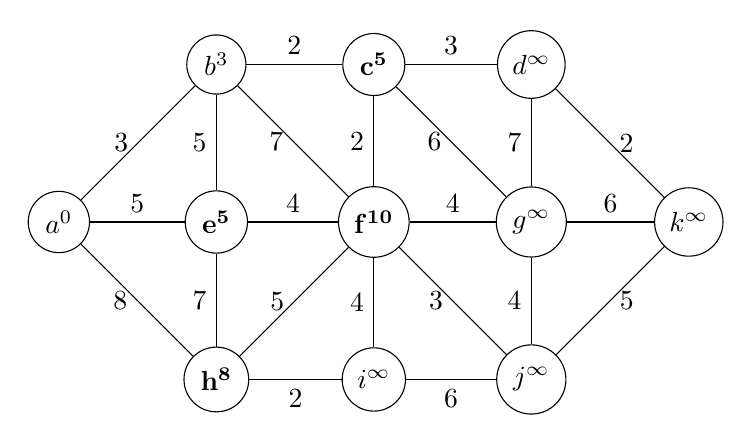
\begin{tikzpicture}
	\node[shape=circle,draw=black] (a) at (0, 2)     {\textbf{$a^0$}};
	\node[shape=circle,draw=black] (b) at (2, 4)     {\textbf{$b^3$}};
	\node[shape=circle,draw=black] (c) at (4, 4)     {\textbf{$\mathbf{c^5}$}};
	\node[shape=circle,draw=black] (d) at (6, 4)     {\textbf{$d^{\infty}$}};
	\node[shape=circle,draw=black] (e) at (2, 2)     {\textbf{$\mathbf{e^5}$}};
	\node[shape=circle,draw=black] (f) at (4, 2)     {\textbf{$\mathbf{f^{10}}$}};
	\node[shape=circle,draw=black] (g) at (6, 2)     {\textbf{$g^{\infty}$}};
	\node[shape=circle,draw=black] (h) at (2, 0)     {\textbf{$\mathbf{h^8}$}};
	\node[shape=circle,draw=black] (i) at (4, 0)     {\textbf{$i^{\infty}$}};
	\node[shape=circle,draw=black] (j) at (6, 0)     {\textbf{$j^{\infty}$}};
	\node[shape=circle,draw=black] (k) at (8, 2)     {\textbf{$k^{\infty}$}};

	\path[-] (a) edge node[left]{3} (b);
	\path[-] (a) edge node[above]{5} (e);
	\path[-] (a) edge node[left]{8} (h);
	\path[-] (b) edge node[left]{5} (e);
	\path[-] (b) edge node[left]{7} (f);
	\path[-] (b) edge node[above]{2} (c);
	\path[-] (e) edge node[above]{4} (f);
	\path[-] (e) edge node[left]{7} (h);
	\path[-] (h) edge node[left]{5} (f);	
	\path[-] (h) edge node[below]{2} (i);	
	\path[-] (c) edge node[above]{3} (d);
	\path[-] (c) edge node[left]{6} (g);
	\path[-] (c) edge node[left]{2} (f);
	\path[-] (f) edge node[above]{4} (g);
	\path[-] (f) edge node[left]{3} (j);
	\path[-] (f) edge node[left]{4} (i);
	\path[-] (i) edge node[below]{6} (j);	
	\path[-] (d) edge node[right]{2} (k);
	\path[-] (d) edge node[left]{7} (g);
	\path[-] (g) edge node[above]{6} (k);
	\path[-] (g) edge node[left]{4} (j);
	\path[-] (j) edge node[right]{5} (k);
	\end{tikzpicture}
\end{figure}

    \begin{itemize}
        \item $b: 3 (a \rightarrow b)$
        \item $e: 5 (a \rightarrow e)$
        \item $h: 8 (a \rightarrow h)$
        \item $c: 5 (a \rightarrow b \rightarrow c)$
        \item $f: 10 (a \rightarrow b \rightarrow f)$
    \end{itemize}{}
    
    Visited nodes: a, b

\pagebreak
    
\item \textbf{Step 3}

Visiting node $e$.

\begin{figure}[H]
	\centering
	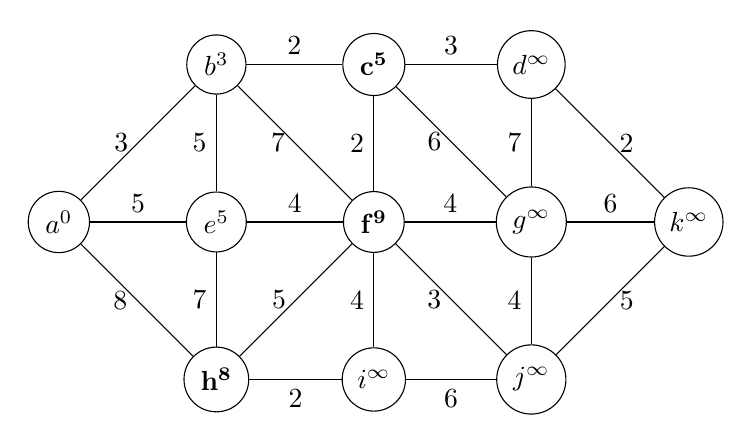
\begin{tikzpicture}
	\node[shape=circle,draw=black] (a) at (0, 2)     {\textbf{$a^0$}};
	\node[shape=circle,draw=black] (b) at (2, 4)     {\textbf{$b^3$}};
	\node[shape=circle,draw=black] (c) at (4, 4)     {\textbf{$\mathbf{c^5}$}};
	\node[shape=circle,draw=black] (d) at (6, 4)     {\textbf{$d^{\infty}$}};
	\node[shape=circle,draw=black] (e) at (2, 2)     {\textbf{$e^5$}};
	\node[shape=circle,draw=black] (f) at (4, 2)     {\textbf{$\mathbf{f^{9}}$}};
	\node[shape=circle,draw=black] (g) at (6, 2)     {\textbf{$g^{\infty}$}};
	\node[shape=circle,draw=black] (h) at (2, 0)     {\textbf{$\mathbf{h^8}$}};
	\node[shape=circle,draw=black] (i) at (4, 0)     {\textbf{$i^{\infty}$}};
	\node[shape=circle,draw=black] (j) at (6, 0)     {\textbf{$j^{\infty}$}};
	\node[shape=circle,draw=black] (k) at (8, 2)     {\textbf{$k^{\infty}$}};

	\path[-] (a) edge node[left]{3} (b);
	\path[-] (a) edge node[above]{5} (e);
	\path[-] (a) edge node[left]{8} (h);
	\path[-] (b) edge node[left]{5} (e);
	\path[-] (b) edge node[left]{7} (f);
	\path[-] (b) edge node[above]{2} (c);
	\path[-] (e) edge node[above]{4} (f);
	\path[-] (e) edge node[left]{7} (h);
	\path[-] (h) edge node[left]{5} (f);	
	\path[-] (h) edge node[below]{2} (i);	
	\path[-] (c) edge node[above]{3} (d);
	\path[-] (c) edge node[left]{6} (g);
	\path[-] (c) edge node[left]{2} (f);
	\path[-] (f) edge node[above]{4} (g);
	\path[-] (f) edge node[left]{3} (j);
	\path[-] (f) edge node[left]{4} (i);
	\path[-] (i) edge node[below]{6} (j);	
	\path[-] (d) edge node[right]{2} (k);
	\path[-] (d) edge node[left]{7} (g);
	\path[-] (g) edge node[above]{6} (k);
	\path[-] (g) edge node[left]{4} (j);
	\path[-] (j) edge node[right]{5} (k);
	\end{tikzpicture}
\end{figure}

    \begin{itemize}
        \item $b: 3 (a \rightarrow b)$
        \item $e: 5 (a \rightarrow e)$
        \item $h: 8 (a \rightarrow h)$
        \item $c: 5 (a \rightarrow b \rightarrow c)$
        \item $f: 9 (a \rightarrow e \rightarrow f)$
    \end{itemize}{}
    
    Visited nodes: a, b, e
    
\item \textbf{Step 4}

Visiting node $h$.

\begin{figure}[H]
	\centering
	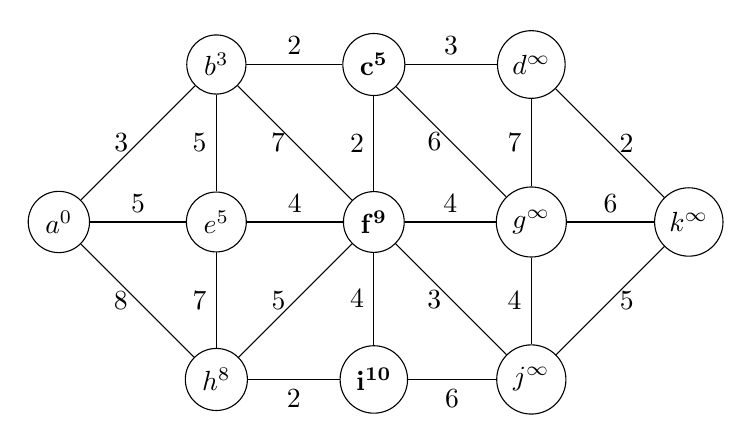
\begin{tikzpicture}
	\node[shape=circle,draw=black] (a) at (0, 2)     {\textbf{$a^0$}};
	\node[shape=circle,draw=black] (b) at (2, 4)     {\textbf{$b^3$}};
	\node[shape=circle,draw=black] (c) at (4, 4)     {\textbf{$\mathbf{c^5}$}};
	\node[shape=circle,draw=black] (d) at (6, 4)     {\textbf{$d^{\infty}$}};
	\node[shape=circle,draw=black] (e) at (2, 2)     {\textbf{$e^5$}};
	\node[shape=circle,draw=black] (f) at (4, 2)     {\textbf{$\mathbf{f^{9}}$}};
	\node[shape=circle,draw=black] (g) at (6, 2)     {\textbf{$g^{\infty}$}};
	\node[shape=circle,draw=black] (h) at (2, 0)     {\textbf{$h^8$}};
	\node[shape=circle,draw=black] (i) at (4, 0)     {\textbf{$\mathbf{i^{10}}$}};
	\node[shape=circle,draw=black] (j) at (6, 0)     {\textbf{$j^{\infty}$}};
	\node[shape=circle,draw=black] (k) at (8, 2)     {\textbf{$k^{\infty}$}};

	\path[-] (a) edge node[left]{3} (b);
	\path[-] (a) edge node[above]{5} (e);
	\path[-] (a) edge node[left]{8} (h);
	\path[-] (b) edge node[left]{5} (e);
	\path[-] (b) edge node[left]{7} (f);
	\path[-] (b) edge node[above]{2} (c);
	\path[-] (e) edge node[above]{4} (f);
	\path[-] (e) edge node[left]{7} (h);
	\path[-] (h) edge node[left]{5} (f);	
	\path[-] (h) edge node[below]{2} (i);	
	\path[-] (c) edge node[above]{3} (d);
	\path[-] (c) edge node[left]{6} (g);
	\path[-] (c) edge node[left]{2} (f);
	\path[-] (f) edge node[above]{4} (g);
	\path[-] (f) edge node[left]{3} (j);
	\path[-] (f) edge node[left]{4} (i);
	\path[-] (i) edge node[below]{6} (j);	
	\path[-] (d) edge node[right]{2} (k);
	\path[-] (d) edge node[left]{7} (g);
	\path[-] (g) edge node[above]{6} (k);
	\path[-] (g) edge node[left]{4} (j);
	\path[-] (j) edge node[right]{5} (k);
	\end{tikzpicture}
\end{figure}

    \begin{itemize}
        \item $b: 3 (a \rightarrow b)$
        \item $e: 5 (a \rightarrow e)$
        \item $h: 8 (a \rightarrow h)$
        \item $c: 5 (a \rightarrow b \rightarrow c)$
        \item $f: 9 (a \rightarrow e \rightarrow f)$
        \item $i: 10 (a \rightarrow h \rightarrow i)$
    \end{itemize}{}
    
    Visited nodes: a, b, e, h
    
\pagebreak
    
\item \textbf{Step 5}

Visiting node $c$.

\begin{figure}[H]
	\centering
	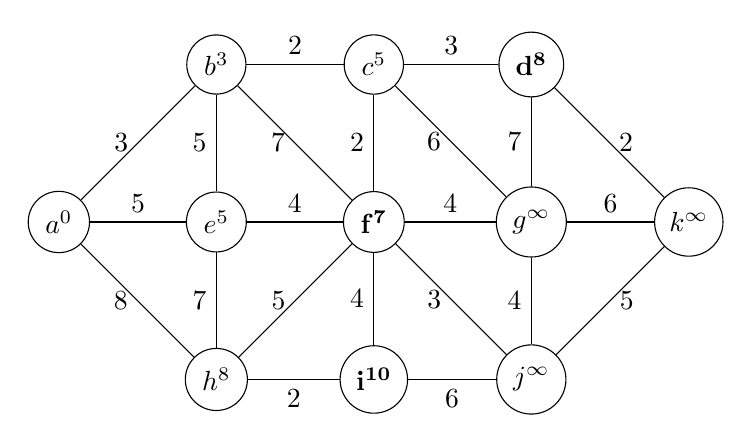
\begin{tikzpicture}
	\node[shape=circle,draw=black] (a) at (0, 2)     {\textbf{$a^0$}};
	\node[shape=circle,draw=black] (b) at (2, 4)     {\textbf{$b^3$}};
	\node[shape=circle,draw=black] (c) at (4, 4)     {\textbf{$c^5$}};
	\node[shape=circle,draw=black] (d) at (6, 4)     {\textbf{$\mathbf{d^8}$}};
	\node[shape=circle,draw=black] (e) at (2, 2)     {\textbf{$e^5$}};
	\node[shape=circle,draw=black] (f) at (4, 2)     {\textbf{$\mathbf{f^{7}}$}};
	\node[shape=circle,draw=black] (g) at (6, 2)     {\textbf{$g^{\infty}$}};
	\node[shape=circle,draw=black] (h) at (2, 0)     {\textbf{$h^8$}};
	\node[shape=circle,draw=black] (i) at (4, 0)     {\textbf{$\mathbf{i^{10}}$}};
	\node[shape=circle,draw=black] (j) at (6, 0)     {\textbf{$j^{\infty}$}};
	\node[shape=circle,draw=black] (k) at (8, 2)     {\textbf{$k^{\infty}$}};

	\path[-] (a) edge node[left]{3} (b);
	\path[-] (a) edge node[above]{5} (e);
	\path[-] (a) edge node[left]{8} (h);
	\path[-] (b) edge node[left]{5} (e);
	\path[-] (b) edge node[left]{7} (f);
	\path[-] (b) edge node[above]{2} (c);
	\path[-] (e) edge node[above]{4} (f);
	\path[-] (e) edge node[left]{7} (h);
	\path[-] (h) edge node[left]{5} (f);	
	\path[-] (h) edge node[below]{2} (i);	
	\path[-] (c) edge node[above]{3} (d);
	\path[-] (c) edge node[left]{6} (g);
	\path[-] (c) edge node[left]{2} (f);
	\path[-] (f) edge node[above]{4} (g);
	\path[-] (f) edge node[left]{3} (j);
	\path[-] (f) edge node[left]{4} (i);
	\path[-] (i) edge node[below]{6} (j);	
	\path[-] (d) edge node[right]{2} (k);
	\path[-] (d) edge node[left]{7} (g);
	\path[-] (g) edge node[above]{6} (k);
	\path[-] (g) edge node[left]{4} (j);
	\path[-] (j) edge node[right]{5} (k);
	\end{tikzpicture}
\end{figure}

    \begin{itemize}
        \item $b: 3 (a \rightarrow b)$
        \item $e: 5 (a \rightarrow e)$
        \item $h: 8 (a \rightarrow h)$
        \item $c: 5 (a \rightarrow b \rightarrow c)$
        \item $f: 7 (a \rightarrow b \rightarrow c \rightarrow f)$
        \item $i: 10 (a \rightarrow h \rightarrow i)$
        \item $d: 8 (a \rightarrow b \rightarrow c \rightarrow d)$
    \end{itemize}{}
    
    Visited nodes: a, b, e, h, c


\item \textbf{Step 6}

Visiting node $f$.

\begin{figure}[H]
	\centering
	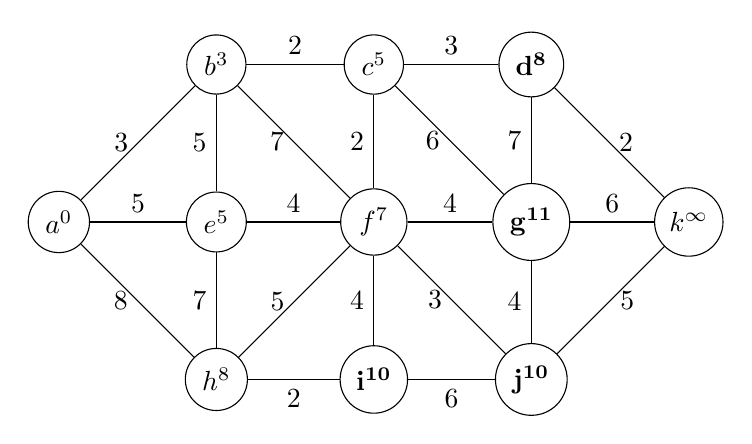
\begin{tikzpicture}
	\node[shape=circle,draw=black] (a) at (0, 2)     {\textbf{$a^0$}};
	\node[shape=circle,draw=black] (b) at (2, 4)     {\textbf{$b^3$}};
	\node[shape=circle,draw=black] (c) at (4, 4)     {\textbf{$c^5$}};
	\node[shape=circle,draw=black] (d) at (6, 4)     {\textbf{$\mathbf{d^8}$}};
	\node[shape=circle,draw=black] (e) at (2, 2)     {\textbf{$e^5$}};
	\node[shape=circle,draw=black] (f) at (4, 2)     {\textbf{$f^{7}$}};
	\node[shape=circle,draw=black] (g) at (6, 2)     {\textbf{$\mathbf{g^{11}}$}};
	\node[shape=circle,draw=black] (h) at (2, 0)     {\textbf{$h^8$}};
	\node[shape=circle,draw=black] (i) at (4, 0)     {\textbf{$\mathbf{i^{10}}$}};
	\node[shape=circle,draw=black] (j) at (6, 0)     {\textbf{$\mathbf{j^{10}}$}};
	\node[shape=circle,draw=black] (k) at (8, 2)     {\textbf{$k^{\infty}$}};

	\path[-] (a) edge node[left]{3} (b);
	\path[-] (a) edge node[above]{5} (e);
	\path[-] (a) edge node[left]{8} (h);
	\path[-] (b) edge node[left]{5} (e);
	\path[-] (b) edge node[left]{7} (f);
	\path[-] (b) edge node[above]{2} (c);
	\path[-] (e) edge node[above]{4} (f);
	\path[-] (e) edge node[left]{7} (h);
	\path[-] (h) edge node[left]{5} (f);	
	\path[-] (h) edge node[below]{2} (i);	
	\path[-] (c) edge node[above]{3} (d);
	\path[-] (c) edge node[left]{6} (g);
	\path[-] (c) edge node[left]{2} (f);
	\path[-] (f) edge node[above]{4} (g);
	\path[-] (f) edge node[left]{3} (j);
	\path[-] (f) edge node[left]{4} (i);
	\path[-] (i) edge node[below]{6} (j);	
	\path[-] (d) edge node[right]{2} (k);
	\path[-] (d) edge node[left]{7} (g);
	\path[-] (g) edge node[above]{6} (k);
	\path[-] (g) edge node[left]{4} (j);
	\path[-] (j) edge node[right]{5} (k);
	\end{tikzpicture}
\end{figure}

    \begin{itemize}
        \item $b: 3 (a \rightarrow b)$
        \item $e: 5 (a \rightarrow e)$
        \item $h: 8 (a \rightarrow h)$
        \item $c: 5 (a \rightarrow b \rightarrow c)$
        \item $f: 7 (a \rightarrow b \rightarrow c \rightarrow f)$
        \item $i: 10 (a \rightarrow h \rightarrow i)$
        \item $d: 8 (a \rightarrow b \rightarrow c \rightarrow d)$
        \item $g: 11 (a \rightarrow e \rightarrow f \rightarrow g)$
        \item $j: 10 (a \rightarrow e \rightarrow f \rightarrow j)$
    \end{itemize}{}
    
    Visited nodes: a, b, e, h, c, f
    
\pagebreak
    
\item \textbf{Step 7}

Visiting node $i$.

\begin{figure}[H]
	\centering
	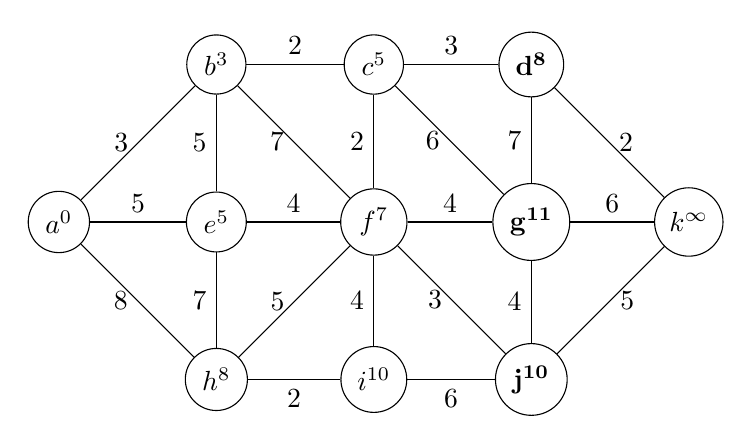
\begin{tikzpicture}
	\node[shape=circle,draw=black] (a) at (0, 2)     {\textbf{$a^0$}};
	\node[shape=circle,draw=black] (b) at (2, 4)     {\textbf{$b^3$}};
	\node[shape=circle,draw=black] (c) at (4, 4)     {\textbf{$c^5$}};
	\node[shape=circle,draw=black] (d) at (6, 4)     {\textbf{$\mathbf{d^8}$}};
	\node[shape=circle,draw=black] (e) at (2, 2)     {\textbf{$e^5$}};
	\node[shape=circle,draw=black] (f) at (4, 2)     {\textbf{$f^{7}$}};
	\node[shape=circle,draw=black] (g) at (6, 2)     {\textbf{$\mathbf{g^{11}}$}};
	\node[shape=circle,draw=black] (h) at (2, 0)     {\textbf{$h^8$}};
	\node[shape=circle,draw=black] (i) at (4, 0)     {\textbf{$i^{10}$}};
	\node[shape=circle,draw=black] (j) at (6, 0)     {\textbf{$\mathbf{j^{10}}$}};
	\node[shape=circle,draw=black] (k) at (8, 2)     {\textbf{$k^{\infty}$}};

	\path[-] (a) edge node[left]{3} (b);
	\path[-] (a) edge node[above]{5} (e);
	\path[-] (a) edge node[left]{8} (h);
	\path[-] (b) edge node[left]{5} (e);
	\path[-] (b) edge node[left]{7} (f);
	\path[-] (b) edge node[above]{2} (c);
	\path[-] (e) edge node[above]{4} (f);
	\path[-] (e) edge node[left]{7} (h);
	\path[-] (h) edge node[left]{5} (f);	
	\path[-] (h) edge node[below]{2} (i);	
	\path[-] (c) edge node[above]{3} (d);
	\path[-] (c) edge node[left]{6} (g);
	\path[-] (c) edge node[left]{2} (f);
	\path[-] (f) edge node[above]{4} (g);
	\path[-] (f) edge node[left]{3} (j);
	\path[-] (f) edge node[left]{4} (i);
	\path[-] (i) edge node[below]{6} (j);	
	\path[-] (d) edge node[right]{2} (k);
	\path[-] (d) edge node[left]{7} (g);
	\path[-] (g) edge node[above]{6} (k);
	\path[-] (g) edge node[left]{4} (j);
	\path[-] (j) edge node[right]{5} (k);
	\end{tikzpicture}
\end{figure}

    \begin{itemize}
        \item $b: 3 (a \rightarrow b)$
        \item $e: 5 (a \rightarrow e)$
        \item $h: 8 (a \rightarrow h)$
        \item $c: 5 (a \rightarrow b \rightarrow c)$
        \item $f: 7 (a \rightarrow b \rightarrow c \rightarrow f)$
        \item $i: 10 (a \rightarrow h \rightarrow i)$
        \item $d: 8 (a \rightarrow b \rightarrow c \rightarrow d)$
        \item $g: 11 (a \rightarrow e \rightarrow f \rightarrow g)$
        \item $j: 10 (a \rightarrow e \rightarrow f \rightarrow j)$
    \end{itemize}{}
    
    Visited nodes: a, b, e, h, c, f, i


\item \textbf{Step 8}

Visiting node $d$.

\begin{figure}[H]
	\centering
	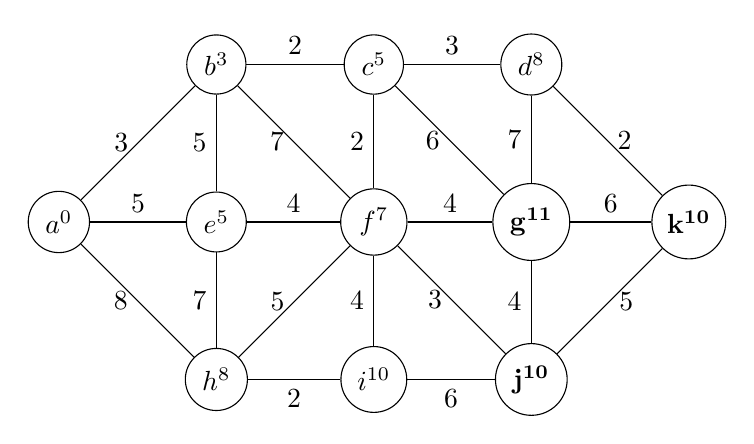
\begin{tikzpicture}
	\node[shape=circle,draw=black] (a) at (0, 2)     {\textbf{$a^0$}};
	\node[shape=circle,draw=black] (b) at (2, 4)     {\textbf{$b^3$}};
	\node[shape=circle,draw=black] (c) at (4, 4)     {\textbf{$c^5$}};
	\node[shape=circle,draw=black] (d) at (6, 4)     {\textbf{$d^8$}};
	\node[shape=circle,draw=black] (e) at (2, 2)     {\textbf{$e^5$}};
	\node[shape=circle,draw=black] (f) at (4, 2)     {\textbf{$f^{7}$}};
	\node[shape=circle,draw=black] (g) at (6, 2)     {\textbf{$\mathbf{g^{11}}$}};
	\node[shape=circle,draw=black] (h) at (2, 0)     {\textbf{$h^8$}};
	\node[shape=circle,draw=black] (i) at (4, 0)     {\textbf{$i^{10}$}};
	\node[shape=circle,draw=black] (j) at (6, 0)     {\textbf{$\mathbf{j^{10}}$}};
	\node[shape=circle,draw=black] (k) at (8, 2)     {\textbf{$\mathbf{k^{10}}$}};

	\path[-] (a) edge node[left]{3} (b);
	\path[-] (a) edge node[above]{5} (e);
	\path[-] (a) edge node[left]{8} (h);
	\path[-] (b) edge node[left]{5} (e);
	\path[-] (b) edge node[left]{7} (f);
	\path[-] (b) edge node[above]{2} (c);
	\path[-] (e) edge node[above]{4} (f);
	\path[-] (e) edge node[left]{7} (h);
	\path[-] (h) edge node[left]{5} (f);	
	\path[-] (h) edge node[below]{2} (i);	
	\path[-] (c) edge node[above]{3} (d);
	\path[-] (c) edge node[left]{6} (g);
	\path[-] (c) edge node[left]{2} (f);
	\path[-] (f) edge node[above]{4} (g);
	\path[-] (f) edge node[left]{3} (j);
	\path[-] (f) edge node[left]{4} (i);
	\path[-] (i) edge node[below]{6} (j);	
	\path[-] (d) edge node[right]{2} (k);
	\path[-] (d) edge node[left]{7} (g);
	\path[-] (g) edge node[above]{6} (k);
	\path[-] (g) edge node[left]{4} (j);
	\path[-] (j) edge node[right]{5} (k);
	\end{tikzpicture}
\end{figure}

    \begin{itemize}
        \item $b: 3 (a \rightarrow b)$
        \item $e: 5 (a \rightarrow e)$
        \item $h: 8 (a \rightarrow h)$
        \item $c: 5 (a \rightarrow b \rightarrow c)$
        \item $f: 7 (a \rightarrow b \rightarrow c \rightarrow f)$
        \item $i: 10 (a \rightarrow h \rightarrow i)$
        \item $d: 8 (a \rightarrow b \rightarrow c \rightarrow d)$
        \item $g: 11 (a \rightarrow e \rightarrow f \rightarrow g)$
        \item $j: 10 (a \rightarrow e \rightarrow f \rightarrow j)$
        \item $k: 10 (a \rightarrow b \rightarrow c \rightarrow d \rightarrow k)$
    \end{itemize}{}
    
    Visited nodes: a, b, e, h, c, f, i, d
    
\item \textbf{Step 9}

Visiting node $g$.

\begin{figure}[H]
	\centering
	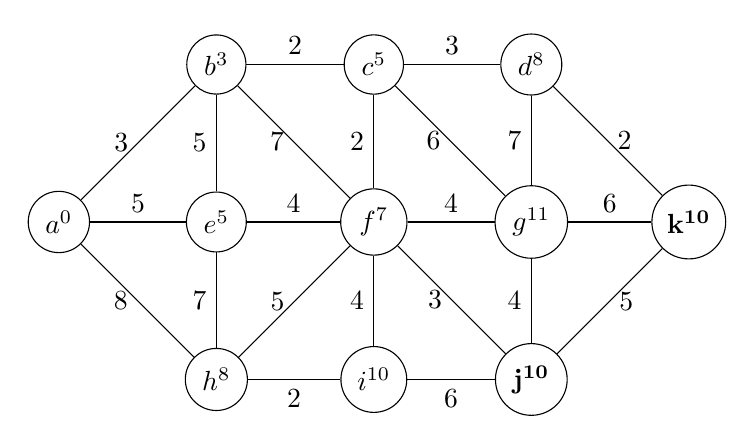
\begin{tikzpicture}
	\node[shape=circle,draw=black] (a) at (0, 2)     {\textbf{$a^0$}};
	\node[shape=circle,draw=black] (b) at (2, 4)     {\textbf{$b^3$}};
	\node[shape=circle,draw=black] (c) at (4, 4)     {\textbf{$c^5$}};
	\node[shape=circle,draw=black] (d) at (6, 4)     {\textbf{$d^8$}};
	\node[shape=circle,draw=black] (e) at (2, 2)     {\textbf{$e^5$}};
	\node[shape=circle,draw=black] (f) at (4, 2)     {\textbf{$f^{7}$}};
	\node[shape=circle,draw=black] (g) at (6, 2)     {\textbf{$g^{11}$}};
	\node[shape=circle,draw=black] (h) at (2, 0)     {\textbf{$h^8$}};
	\node[shape=circle,draw=black] (i) at (4, 0)     {\textbf{$i^{10}$}};
	\node[shape=circle,draw=black] (j) at (6, 0)     {\textbf{$\mathbf{j^{10}}$}};
	\node[shape=circle,draw=black] (k) at (8, 2)     {\textbf{$\mathbf{k^{10}}$}};

	\path[-] (a) edge node[left]{3} (b);
	\path[-] (a) edge node[above]{5} (e);
	\path[-] (a) edge node[left]{8} (h);
	\path[-] (b) edge node[left]{5} (e);
	\path[-] (b) edge node[left]{7} (f);
	\path[-] (b) edge node[above]{2} (c);
	\path[-] (e) edge node[above]{4} (f);
	\path[-] (e) edge node[left]{7} (h);
	\path[-] (h) edge node[left]{5} (f);	
	\path[-] (h) edge node[below]{2} (i);	
	\path[-] (c) edge node[above]{3} (d);
	\path[-] (c) edge node[left]{6} (g);
	\path[-] (c) edge node[left]{2} (f);
	\path[-] (f) edge node[above]{4} (g);
	\path[-] (f) edge node[left]{3} (j);
	\path[-] (f) edge node[left]{4} (i);
	\path[-] (i) edge node[below]{6} (j);	
	\path[-] (d) edge node[right]{2} (k);
	\path[-] (d) edge node[left]{7} (g);
	\path[-] (g) edge node[above]{6} (k);
	\path[-] (g) edge node[left]{4} (j);
	\path[-] (j) edge node[right]{5} (k);
	\end{tikzpicture}
\end{figure}

    \begin{itemize}
        \item $b: 3 (a \rightarrow b)$
        \item $e: 5 (a \rightarrow e)$
        \item $h: 8 (a \rightarrow h)$
        \item $c: 5 (a \rightarrow b \rightarrow c)$
        \item $f: 7 (a \rightarrow b \rightarrow c \rightarrow f)$
        \item $i: 10 (a \rightarrow h \rightarrow i)$
        \item $d: 8 (a \rightarrow b \rightarrow c \rightarrow d)$
        \item $g: 11 (a \rightarrow e \rightarrow f \rightarrow g)$
        \item $j: 10 (a \rightarrow e \rightarrow f \rightarrow j)$
        \item $k: 10 (a \rightarrow b \rightarrow c \rightarrow d \rightarrow k)$
    \end{itemize}{}
    
    Visited nodes: a, b, e, h, c, f, i, d, g

\pagebreak

\item \textbf{Step 10}

Visiting node $j$.

\begin{figure}[H]
	\centering
	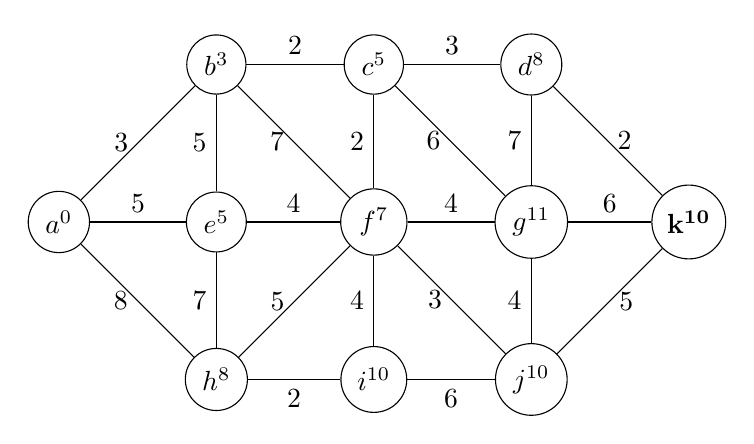
\begin{tikzpicture}
	\node[shape=circle,draw=black] (a) at (0, 2)     {\textbf{$a^0$}};
	\node[shape=circle,draw=black] (b) at (2, 4)     {\textbf{$b^3$}};
	\node[shape=circle,draw=black] (c) at (4, 4)     {\textbf{$c^5$}};
	\node[shape=circle,draw=black] (d) at (6, 4)     {\textbf{$d^8$}};
	\node[shape=circle,draw=black] (e) at (2, 2)     {\textbf{$e^5$}};
	\node[shape=circle,draw=black] (f) at (4, 2)     {\textbf{$f^{7}$}};
	\node[shape=circle,draw=black] (g) at (6, 2)     {\textbf{$g^{11}$}};
	\node[shape=circle,draw=black] (h) at (2, 0)     {\textbf{$h^8$}};
	\node[shape=circle,draw=black] (i) at (4, 0)     {\textbf{$i^{10}$}};
	\node[shape=circle,draw=black] (j) at (6, 0)     {\textbf{$j^{10}$}};
	\node[shape=circle,draw=black] (k) at (8, 2)     {\textbf{$\mathbf{k^{10}}$}};

	\path[-] (a) edge node[left]{3} (b);
	\path[-] (a) edge node[above]{5} (e);
	\path[-] (a) edge node[left]{8} (h);
	\path[-] (b) edge node[left]{5} (e);
	\path[-] (b) edge node[left]{7} (f);
	\path[-] (b) edge node[above]{2} (c);
	\path[-] (e) edge node[above]{4} (f);
	\path[-] (e) edge node[left]{7} (h);
	\path[-] (h) edge node[left]{5} (f);	
	\path[-] (h) edge node[below]{2} (i);	
	\path[-] (c) edge node[above]{3} (d);
	\path[-] (c) edge node[left]{6} (g);
	\path[-] (c) edge node[left]{2} (f);
	\path[-] (f) edge node[above]{4} (g);
	\path[-] (f) edge node[left]{3} (j);
	\path[-] (f) edge node[left]{4} (i);
	\path[-] (i) edge node[below]{6} (j);	
	\path[-] (d) edge node[right]{2} (k);
	\path[-] (d) edge node[left]{7} (g);
	\path[-] (g) edge node[above]{6} (k);
	\path[-] (g) edge node[left]{4} (j);
	\path[-] (j) edge node[right]{5} (k);
	\end{tikzpicture}
\end{figure}

    \begin{itemize}
        \item $b: 3 (a \rightarrow b)$
        \item $e: 5 (a \rightarrow e)$
        \item $h: 8 (a \rightarrow h)$
        \item $c: 5 (a \rightarrow b \rightarrow c)$
        \item $f: 7 (a \rightarrow b \rightarrow c \rightarrow f)$
        \item $i: 10 (a \rightarrow h \rightarrow i)$
        \item $d: 8 (a \rightarrow b \rightarrow c \rightarrow d)$
        \item $g: 11 (a \rightarrow e \rightarrow f \rightarrow g)$
        \item $j: 10 (a \rightarrow e \rightarrow f \rightarrow j)$
        \item $k: 10 (a \rightarrow b \rightarrow c \rightarrow d \rightarrow k)$
    \end{itemize}{}
    
    Visited nodes: a, b, e, h, c, f, i, d, g, j

\item \textbf{Step 11}

Visiting node $k$.

\begin{figure}[H]
	\centering
	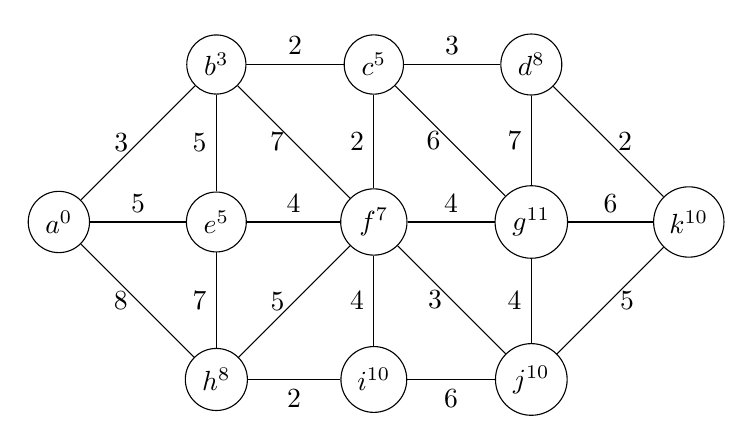
\begin{tikzpicture}
	\node[shape=circle,draw=black] (a) at (0, 2)     {\textbf{$a^0$}};
	\node[shape=circle,draw=black] (b) at (2, 4)     {\textbf{$b^3$}};
	\node[shape=circle,draw=black] (c) at (4, 4)     {\textbf{$c^5$}};
	\node[shape=circle,draw=black] (d) at (6, 4)     {\textbf{$d^8$}};
	\node[shape=circle,draw=black] (e) at (2, 2)     {\textbf{$e^5$}};
	\node[shape=circle,draw=black] (f) at (4, 2)     {\textbf{$f^{7}$}};
	\node[shape=circle,draw=black] (g) at (6, 2)     {\textbf{$g^{11}$}};
	\node[shape=circle,draw=black] (h) at (2, 0)     {\textbf{$h^8$}};
	\node[shape=circle,draw=black] (i) at (4, 0)     {\textbf{$i^{10}$}};
	\node[shape=circle,draw=black] (j) at (6, 0)     {\textbf{$j^{10}$}};
	\node[shape=circle,draw=black] (k) at (8, 2)     {\textbf{$k^{10}$}};

	\path[-] (a) edge node[left]{3} (b);
	\path[-] (a) edge node[above]{5} (e);
	\path[-] (a) edge node[left]{8} (h);
	\path[-] (b) edge node[left]{5} (e);
	\path[-] (b) edge node[left]{7} (f);
	\path[-] (b) edge node[above]{2} (c);
	\path[-] (e) edge node[above]{4} (f);
	\path[-] (e) edge node[left]{7} (h);
	\path[-] (h) edge node[left]{5} (f);	
	\path[-] (h) edge node[below]{2} (i);	
	\path[-] (c) edge node[above]{3} (d);
	\path[-] (c) edge node[left]{6} (g);
	\path[-] (c) edge node[left]{2} (f);
	\path[-] (f) edge node[above]{4} (g);
	\path[-] (f) edge node[left]{3} (j);
	\path[-] (f) edge node[left]{4} (i);
	\path[-] (i) edge node[below]{6} (j);	
	\path[-] (d) edge node[right]{2} (k);
	\path[-] (d) edge node[left]{7} (g);
	\path[-] (g) edge node[above]{6} (k);
	\path[-] (g) edge node[left]{4} (j);
	\path[-] (j) edge node[right]{5} (k);
	\end{tikzpicture}
\end{figure}

    \begin{itemize}
        \item $b: 3 (a \rightarrow b)$
        \item $e: 5 (a \rightarrow e)$
        \item $h: 8 (a \rightarrow h)$
        \item $c: 5 (a \rightarrow b \rightarrow c)$
        \item $f: 7 (a \rightarrow b \rightarrow c \rightarrow f)$
        \item $i: 10 (a \rightarrow h \rightarrow i)$
        \item $d: 8 (a \rightarrow b \rightarrow c \rightarrow d)$
        \item $g: 11 (a \rightarrow e \rightarrow f \rightarrow g)$
        \item $j: 10 (a \rightarrow e \rightarrow f \rightarrow j)$
        \item $k: 10 (a \rightarrow b \rightarrow c \rightarrow d \rightarrow k)$
    \end{itemize}{}
    
    Visited nodes: a, b, e, h, c, f, i, d, g, j, k

\item \textbf{Step 12}

    Since there is no unvisited vertex left, the Djikstra algorithm has finished. The shortest path from $a$ to $j$ is the path $(a \rightarrow e \rightarrow f \rightarrow j)$ with the cost 10.

\end{itemize}{}
    
\subsection*{b)}
    \begin{table}[H]
        \centering
        \begin{tabular}{c|c|c}
             Choice & Edge & Weight \\
             \hline
             1  & \texttt{\{a,b\}} & 3 \\
             2  & \texttt{\{b,c\}} & 2 \\
             3  & \texttt{\{c,f\}} & 2 \\
             4  & \texttt{\{e,f\}} & 4 \\
             5  & \texttt{\{f,i\}} & 4 \\
             6  & \texttt{\{h,i\}} & 2 \\
             7  & \texttt{\{f,j\}} & 3 \\
             8  & \texttt{\{g,j\}} & 4 \\
             9  & \texttt{\{c,d\}} & 3 \\
             10 & \texttt{\{d,k\}} & 2
        \end{tabular}
        ~ \\
        ~ \\
        Total: 29
    \end{table}{}
    
    

    \begin{figure}[H]
	\centering
	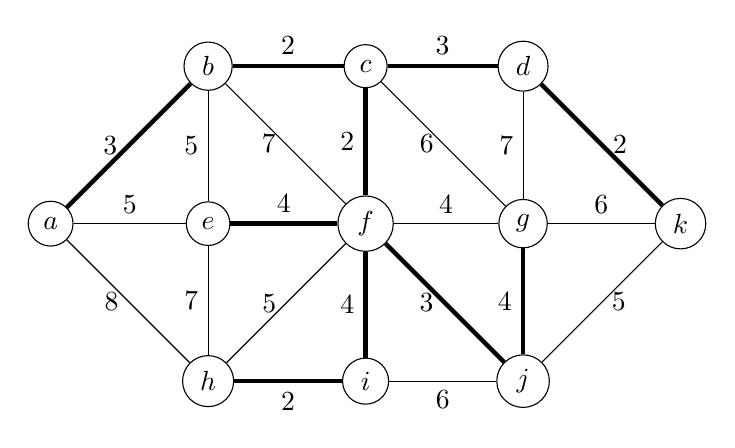
\begin{tikzpicture}
	\node[shape=circle,draw=black] (a) at (0, 2)     {\textbf{$a$}};
	\node[shape=circle,draw=black] (b) at (2, 4)     {\textbf{$b$}};
	\node[shape=circle,draw=black] (c) at (4, 4)     {\textbf{$c$}};
	\node[shape=circle,draw=black] (d) at (6, 4)     {\textbf{$d$}};
	\node[shape=circle,draw=black] (e) at (2, 2)     {\textbf{$e$}};
	\node[shape=circle,draw=black] (f) at (4, 2)     {\textbf{$f$}};
	\node[shape=circle,draw=black] (g) at (6, 2)     {\textbf{$g$}};
	\node[shape=circle,draw=black] (h) at (2, 0)     {\textbf{$h$}};
	\node[shape=circle,draw=black] (i) at (4, 0)     {\textbf{$i$}};
	\node[shape=circle,draw=black] (j) at (6, 0)     {\textbf{$j$}};
	\node[shape=circle,draw=black] (k) at (8, 2)     {\textbf{$k$}};

	\path[ultra thick] (a) edge node[left]{3} (b);
	\path[-] (a) edge node[above]{5} (e);
	\path[-] (a) edge node[left]{8} (h);
	\path[-] (b) edge node[left]{5} (e);
	\path[-] (b) edge node[left]{7} (f);
	\path[ultra thick] (b) edge node[above]{2} (c);
	\path[ultra thick] (e) edge node[above]{4} (f);
	\path[-] (e) edge node[left]{7} (h);
	\path[-] (h) edge node[left]{5} (f);	
	\path[ultra thick] (h) edge node[below]{2} (i);	
	\path[ultra thick] (c) edge node[above]{3} (d);
	\path[-] (c) edge node[left]{6} (g);
	\path[ultra thick] (c) edge node[left]{2} (f);
	\path[-] (f) edge node[above]{4} (g);
	\path[ultra thick] (f) edge node[left]{3} (j);
	\path[ultra thick] (f) edge node[left]{4} (i);
	\path[-] (i) edge node[below]{6} (j);	
	\path[ultra thick] (d) edge node[right]{2} (k);
	\path[-] (d) edge node[left]{7} (g);
	\path[-] (g) edge node[above]{6} (k);
	\path[ultra thick] (g) edge node[left]{4} (j);
	\path[-] (j) edge node[right]{5} (k);
	\end{tikzpicture}
\end{figure}

\section*{Answer 6}

\subsection*{a)} 
    There are $\mathbf{7}$ vertices, $\mathbf{6}$ edges on T. It's height is $\mathbf{3}$.

\subsection*{b)}
    \texttt{a:17 b:13 c:24 d:19 e:43 f:23 g:58}

\subsection*{c)}
    \texttt{b:13 d:19 f:23 g:58 e:43 c:24 a:17}
    
\subsection*{d)}
    \texttt{b:13 a:17 d:19 c:24 f:23 e:43 g:58 }

\subsection*{e)}
    \begin{itemize}
        \item Definition 3 from section 11.1 of the textbook says, "The tree is called a full m-ary tree if every internal vertex has exactly m children. An m-ary tree with m = 2 is called a binary tree."
        \item So in order to T be a full binary tree, every non-leaf node has exactly 2 children.
        \item Non-leaf nodes, namely \texttt{a, c, e}, has exactly 2 children. As a result, T is a full binary tree.
    \end{itemize}{}
    
\subsection*{f)}
    \begin{itemize}
        \item Section 11.1 of the textbook says: "A complete m-ary tree is a full m-ary tree in which every leaf is at the same level."
        \item We know from the part e that the tree T is a full binary tree.
        \item In order to T be a complete binary tree, all leaves must be at same level. But leaves \texttt{d and f} are not in the same level. Hence, the tree T is not a complete binary tree.
    \end{itemize}{}
    
\subsection*{g)}
    \begin{itemize}
        \item In a binary search tree, if we do a inorder traversal the values of the vertices must be in ordered. (Since in inorder traversal, the order follows left-middle-right, and in a binary search tree middle values always greater than left values and always smaller than right values).
        \item From the part d, we can see that the vertices \texttt{c and f} are not in order. Hence, T is not a binary search tree.
    \end{itemize}{}
    
\subsection*{h)}
    \begin{itemize}
        \item In order to the graph be a full binary tree, all nodes except leaves must have exactly two children.
        \item For that purpose, for every non-leaf node must have one leaf and one non-leaf node except the nodes at level 5. This is the only way to both increase the height of the three same as following the rules for full-binary tree.
        \item So, in every level of the binary-tree there must be two nodes, except the root node. So we can create a formula for the minimum number of nodes in order to create a full binary tree as $node\_count = 2 \cdot h + 1$.
        \item Hence, the minimum number of nodes to create full binary tree with height 5 is, $2 * 5 + 1 = 11$.
        
        \begin{figure}[H]
        	\centering
        	\begin{tikzpicture}
        	
        	\node[shape=circle,draw=black] (a) at (5, 5) {\textbf{}};
        	\node[shape=circle,draw=black] (b) at (4, 4) {\textbf{}};
        	\node[shape=circle,draw=black] (c) at (6, 4) {\textbf{}};
        	\node[shape=circle,draw=black] (d) at (3, 3) {\textbf{}};
        	\node[shape=circle,draw=black] (e) at (5, 3) {\textbf{}};
        	\node[shape=circle,draw=black] (f) at (2, 2) {\textbf{}};
        	\node[shape=circle,draw=black] (g) at (4, 2) {\textbf{}};
        	\node[shape=circle,draw=black] (h) at (1, 1) {\textbf{}};
        	\node[shape=circle,draw=black] (i) at (3, 1) {\textbf{}};
        	\node[shape=circle,draw=black] (j) at (0, 0) {\textbf{}};
        	\node[shape=circle,draw=black] (k) at (2, 0) {\textbf{}};
        	
        	\path[-] (a) edge (b);
        	\path[-] (a) edge (c);
        	\path[-] (b) edge (d);
            \path[-] (b) edge (e);
            \path[-] (d) edge (f);
            \path[-] (d) edge (g);
            \path[-] (f) edge (h);
            \path[-] (f) edge (i);
            \path[-] (h) edge (j);
            \path[-] (h) edge (k);
            
        	\end{tikzpicture} 
        \end{figure}
    \end{itemize}{}
    
\subsection*{i)}

\begin{figure}[H]
	\centering
	\begin{tikzpicture}
	
	\node[shape=circle,draw=black] (a) at (6, 4)     {\textbf{4}};
	\node[shape=circle,draw=black] (b) at (3, 2)     {\textbf{2}};
	\node[shape=circle,draw=black] (c) at (9, 2)   {\textbf{6}};
	
	\node[shape=circle,draw=black] (d) at (1, 0)     {\textbf{1}};
	\node[shape=circle,draw=black] (e) at (5, 0)     {\textbf{3}};
	\node[shape=circle,draw=black] (f) at (8, 0)    {\textbf{5}};
	
	\path[-] (a) edge (b);
	\path[-] (a) edge (c);
	\path[-] (b) edge (d);
	\path[-] (b) edge (e);
	\path[-] (c) edge (f);

	\end{tikzpicture} 
\end{figure}

\subsection*{j)}
    \begin{itemize}
        \item Sequence to find 1: $4 \xrightarrow{\text{left}} 2 \xrightarrow{\text{left}} 1$
        \item Sequence to find 6: $4 \xrightarrow{\text{right}} 6$
    \end{itemize}{}
    
\subsection*{k)}
    \begin{figure}[H]
    	\centering
    	\begin{tikzpicture}
    	
    	\node[shape=circle,draw=black] (d) at (6, 4)   {\textbf{d}};
    	\node[shape=circle,draw=black] (e) at (2, 2)   {\textbf{e}};
    	\node[shape=circle,draw=black] (c) at (5, 2)   {\textbf{c}};
    	\node[shape=circle,draw=black] (b) at (8, 2)   {\textbf{b}};
    	\node[shape=circle,draw=black] (a) at (11, 2)   {\textbf{a}};
    	
    	\node[shape=circle,draw=black] (g) at (0, 0)   {\textbf{g}};
    	\node[shape=circle,draw=black] (f) at (4, 0)   {\textbf{f}};
    	
    	\path[-] (d) edge (e);
    	\path[-] (d) edge (c);
    	\path[-] (d) edge (a);
    	\path[-] (d) edge (b);
    	
    	\path[-] (e) edge (g);
    	\path[-] (e) edge (f);
    
    	\end{tikzpicture} 
    \end{figure}
    
\subsection*{l)}
    \begin{itemize}
        \item If we want to have maximum height from the binary search tree, we can put only one vertex in every level of the binary tree. Using this method, we can generate tree with height $k - 1$ using $k$ vertices.
        \item Let's take the set $S = \{1, 2, 3, 4, 5, 6\}$. If we want to create a binary search tree with maximum height, we can put these vertices like below.
        
        \begin{figure}[H]
        	\centering
        	\begin{tikzpicture}
        	
        	\node[shape=circle,draw=black] (a) at (5, 5) {\textbf{6}};
        	\node[shape=circle,draw=black] (b) at (4, 4) {\textbf{5}};
        	\node[shape=circle,draw=black] (c) at (3, 3) {\textbf{4}};
        	\node[shape=circle,draw=black] (d) at (2, 2) {\textbf{3}};
        	\node[shape=circle,draw=black] (e) at (1, 1) {\textbf{2}};
        	\node[shape=circle,draw=black] (f) at (0, 0) {\textbf{1}};
        	
        	\path[-] (a) edge (b);
        	\path[-] (b) edge (c);
            \path[-] (c) edge (d);
            \path[-] (d) edge (e);
            \path[-] (e) edge (f);
            
        	\end{tikzpicture} 
        \end{figure}
        \item Since every level of binary search tree must be have at least one vertex, this is the only way to create binary search tree with maximum height. We cannot increase the height more without removing any of the level, which it is changes nothing if it removes a level from the binary search tree.
        \item Hence, using $k$ vertex, binary search tree with maximum $k-1$ height can be generated.
    \end{itemize}{}

\end{document}
